\documentclass[a4paper, 12pt]{article}
\usepackage{fullpage}
\usepackage[utf8]{inputenc}
\usepackage[english]{babel}
\usepackage{latexsym}
\usepackage{color}
\usepackage{amssymb}
\usepackage{amsmath}
\usepackage{graphicx}
\usepackage{fancyhdr}

\pagestyle{fancy}
\fancyhf{}
\fancyhead[RE,LO]{Project 2: Learning of Grid Cells}
\headsep=15mm

\title{Project 2: Learning of Grid Cells}
\author{Claus Lang, Can Eren Sezener, Claudia Winklmayr}
\date{09.02.2016}


\begin{document}
\maketitle

\paragraph{Abstract:}
Grid cells, located in rats medial entorhinal cortex (mEC), show increased fireing activity when the animal enters specific regions of the environment. The resulting firing maps show a characteristic hexagonal grid pattern. In our project we implement a computational model for the developement of grid cells, introduced by Kropff and Treves. We simulate a rat exploring a square environment. The $x$ and $y$ coordinates of its loactions serve as input for a layer of 40 place unitis. The output layer then recieves a weighted sum of the places cell activity to compute the grid cell activation. Weights are updated by a Hebbinan learning rule. 

\section{Introduction}
There are various types of neurons that serve to encode an animals spacial location. Place cells- located in hippocampus- were discovered in the 1970s by O'Keefe and Dostrovsky. Place cells show increased activity when the animal enters a specific region of the environment- the so called place field.\newline
Grid cells - located in medial entorhinal cortex (mEC) werde then discovered in 2005. In contrast to place cells they are activated at various locations and their firing maps show a characteristic hexagonal grid pattern. Different grid cells can be distingusihed by their spacing, orientation and spacial phases and neighbouring grid cells show similar and orientation. \newline
It is assumed that grid cells perfom a path integration task, taking into account the rats position, speed and direction. Visual information on the other hand plays at most a secondary role in the formation of the grid pattern. \newline
The Kropff and Treves model assumes places cells as the basis for grid cell developement. The place cells take as imput the $x$ and $y$ coordiantes of a virtual rat exploring a square environment of 125cm length. Every output unit then recieves input from all place cells and the weights connecting input and output neurons are updated by a Hebbian learning rule. 
%
%
%
\section{Model}
%
%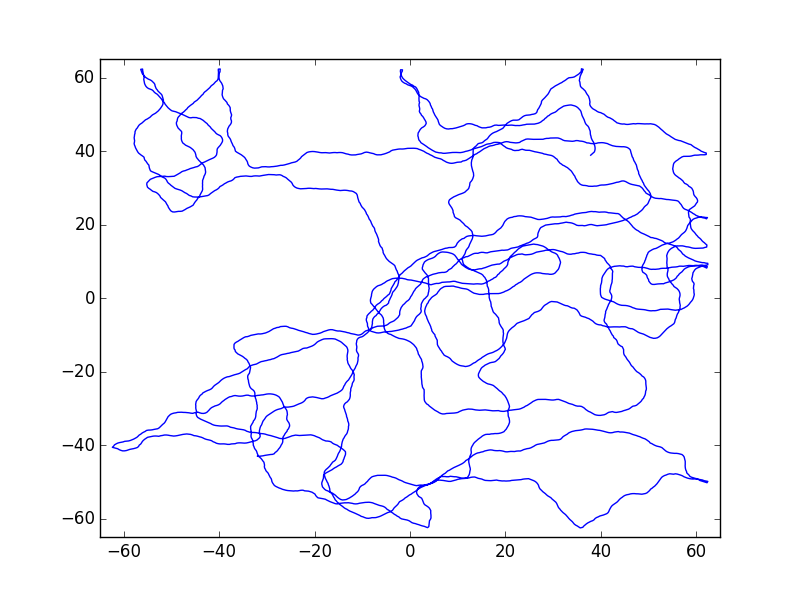
\includegraphics[width=6cm]{running_rat.png}
%\caption{running time: 50 seconds}


%
%
%
\section{Results}
%


\subsection{Time evolution}
\begin{figure}[htbp]
\begin{minipage}[hbt]{0,49\textwidth}
        \centering
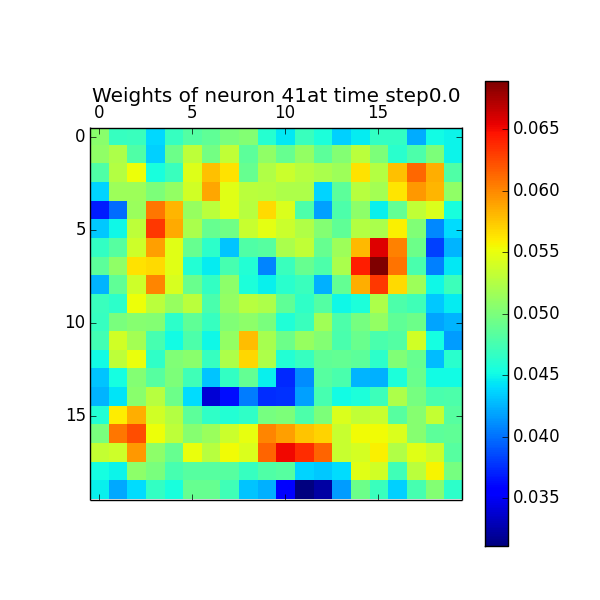
\includegraphics[width=6cm,height=6cm]{neurons/neuron_w_41_t_0.png}\\[10pt]
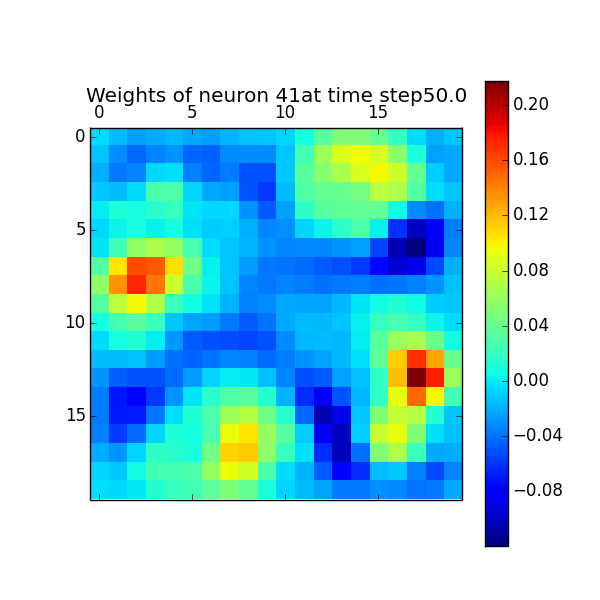
\includegraphics[width=6cm,height=6cm]{neurons/neuron_w_41_t_50.png} \\[10pt]
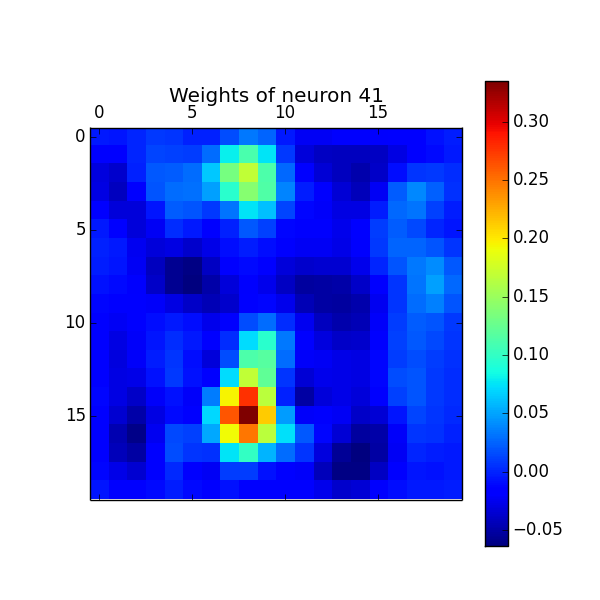
\includegraphics[width=6cm,height=6cm]{neurons/neuron_w_41.png}
        \caption{weight developement}
        \label{LabelA}
\end{minipage}
\begin{minipage}[hbt]{0,49\textwidth}
        \centering
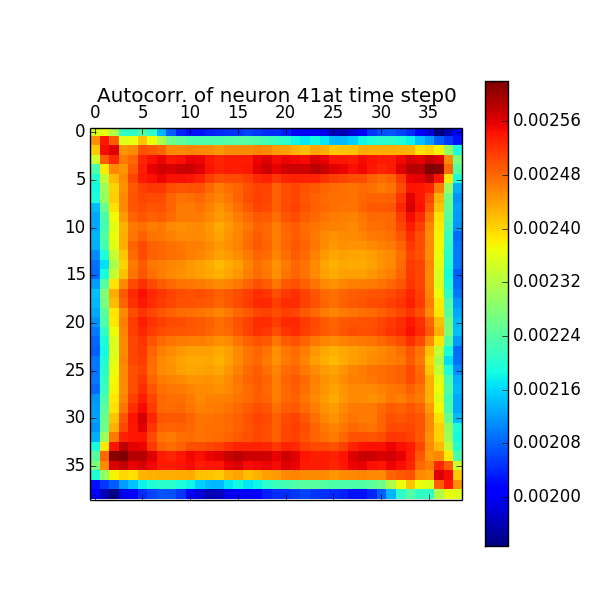
\includegraphics[width=6cm,height=6cm]{neurons/neuron_a_41_t_0.png}\\[10pt]
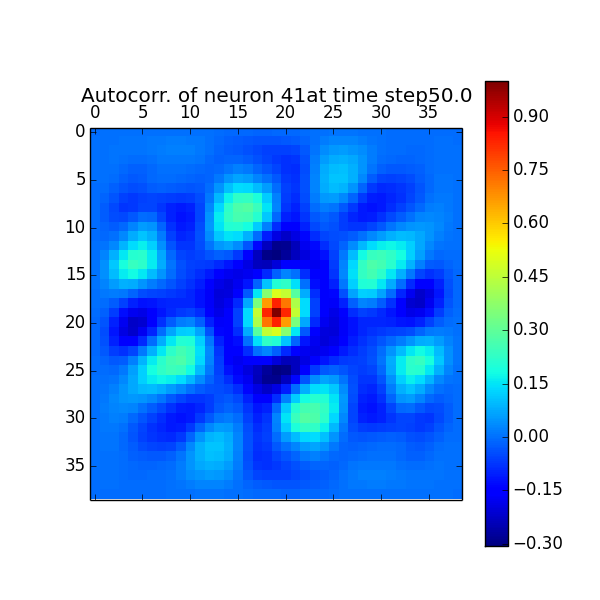
\includegraphics[width=6cm,height=6cm]{neurons/neuron_a_41_t_50.png}\\[10pt]
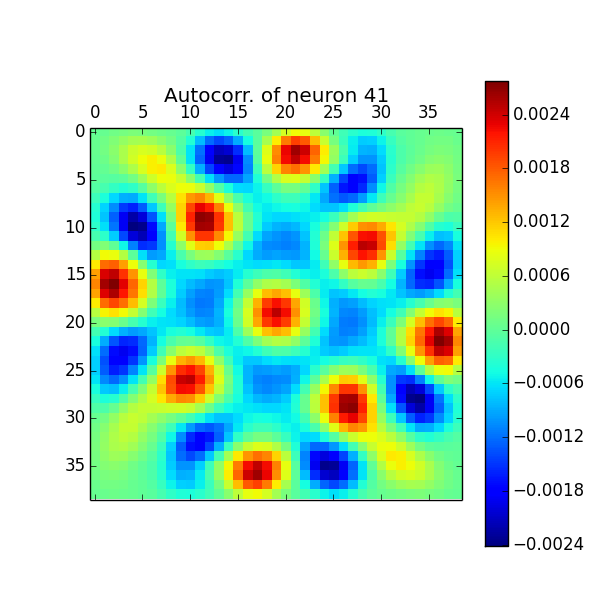
\includegraphics[width=6cm,height=6cm]{neurons/neuron_a_41.png}
        \caption{autocorrellation developement}
        \label{LabelB}
\end{minipage}
\centering
\caption{Developement }
\end{figure}

\section{References}

\end{document}

	